\chapter{Cone}
%

% - Purpose & Problem description:
%     These first two parts give reader short details about the test case,
%     the physical phenomena involved and specify how the numerical solution will be validated
\section{Description of the problem}
%
%purpose
This test shows the performance of the advection schemes of \telemac{2d} for passive scalar transport in a time dependent case. \\
%
It shows the advection of a tracer (or any other passive scalar) in a square basin of dimensions $[d \times d]=[20.1 \times 20.1]~m^2$ with flat frictionless bottom and with open boundaries. The tracer is described by a gaussian function and is submitted to a rotating velocity field. In this case the scalar advection equation is solved using fixed hydrodynamic conditions. After one period we expect that the tracer function have the same position and the same values as the initial condition (i.e. maximum value equal to 1 at the center). The exact solution can indeed be computed using the theory of characteristics. \\
In order to evaluate the behaviour of the scheme, the error norms $L^1, L^2, L^{\infty}$ and the maximum value of the gaussian function are measured after one rotation. The minimum value is computed as well, in order to check the respect of the maximum principle (or monotonicity). \\
The water depth is constant in time and in space, equal to $2~m$. The velocity field is constant in time as well and is divergence free:
\begin{equation*}
  \vec{u}=\left\{
         \begin{array}{l}
          u(x,y)=-(y-d/2) \\
          v(x,y)=(x-d/2)
         \end{array}\right.
\end{equation*}
The initial condition for the tracer is:
\begin{equation*}
 c^0(x,y)=e^{-\frac{[(x-15)^2+(y-10.2)^2]}{2}}
\end{equation*}
where $c$ represents the concentration of the tracer. \\
%which bounds the solution between 0 and 1.
The simulation time is one period of rotation equal to $2\pi$, that is $6.28~s$.
% - Numerical parameters:
%     This part is used to specify the numerical parameters used
%     (adaptive time step, mass-lumping when necessary...)
%
%
\section{Numerical parameters}
%
The computationl domain for this test is made up by squares of side $0.3~m$ split into two triangles.
The number of nodes is 4624 and the number of element is 8978.
The time step is chosen in order to do the whole period in 32 steps, so it is equal to $0.196349541~s$.
%However this test is not suitable to check mass conservation (due to the open boundaries where hydrodynamics is not solved).
\\
For tracers advection, all the numerical schemes available in \telemac{2d} are tested. \\
For weak characteristics the number of gauss points is set to 12. For distributive schemes, like predictor-corrector (PC) schemes (scheme 4 and 5 with options 2,3) and locally implicit schemes (LIPS: scheme 4 and 5 with options 4), the number of correction is set to 5, which is usually sufficient to converge to accurate results. For the locally implicit schemes (scheme 4 and 5 with option 4), the number of sub-steps is equal to 20.
%
% - Results:
%     We comment in this part the numerical results against the reference ones,
%     giving understanding keys and making assumptions when necessary.
%
%
\section{Results}
The error norms, the maximum and the minimum value of the tracer function at the end of the simulation are reported in Table \ref{t2d:cone:tab1}. The final profiles for every schemes are plotted in Figures \ref{t2d:cone:profiles1} and \ref{t2d:cone:profiles2}. Schemes can be listed from the most most accurate to the least accurate: weak characteristics, N LIPS, PSI LIPS (these two are overlapped), ERIA, PSI PC1, N PC1, strong characteristics, PSI PC2, N PC2, PSI, N.
The error computations of Table \ref{t2d:cone:tab1} are in agreement with the figures.\\
However, it is worth noticing that the weak characteristics give the highest maximum value but the scheme does not guarantee the maximum principle, indeed negative values are produced along the simulation (this is also visible on the Figure \ref{t2d:cone:profiles1} and in Table \ref{t2d:cone:tab1}). On the contrary, all the distributive schemes guarantee the respect of the maximum principle: minimum and maximum extrema are never exceeded. \\
\telemac{2d} is able to model passive scalar transport problems in shallow water flows. This test shows that to get higher accuracy and monotonicity in passive scalar transport cases the predictor-corrector distributive schemes (N PC, PSI PC or LIPS) are the most appropriate schemes, as well as the ERIA scheme.
%
\begin{table}[H]
\centering
\caption{Cone test: error norms and extrema at the end of the simulation.}
\begin{tabular}{l|}
\\ \hline Strong characteristics \\ Weak characteristics \\ ERIA \\ N \\ N LIPS \\ PSI \\ PSI PC1 \\ PSI PC2 \\ N PC1 \\ N PC2 \\ PSI LIPS
\end{tabular}%
\begin{tabular}{|c|c|c|c|c}
  $||\epsilon||_{L^1}$ & $||\epsilon||_{L^2}$ & $||\epsilon||_{L^{\infty}}$ & $\min(c)$ & $\max(c)$\\
\hline
\input{../table.txt}
\label{t2d:cone:tab1}
\end{tabular}
\end{table}
%\preparetable {../table.txt}{1, 2, 3, 4, 5, 6, 7, 8, 9, 10, 11}
%\begin{tabular}{ccccc}
%\usetable
%\end{tabular}
% Images should be in test_case/img
% just an example
%\begin{figure}[h!]
%\centering
%\includegraphics[width=\textwidth]{../img/figure_1d.pdf}
%\caption{Cone test: final results at section y=10.2 for 5$\le$ x$\le$20.1 for all advection schemes of \telemac{2d}.}
%\label{t2d:cone:1d}
%\end{figure}
\begin{figure}[h!]
\begin{minipage}[t]{0.50\textwidth}
 \centering
 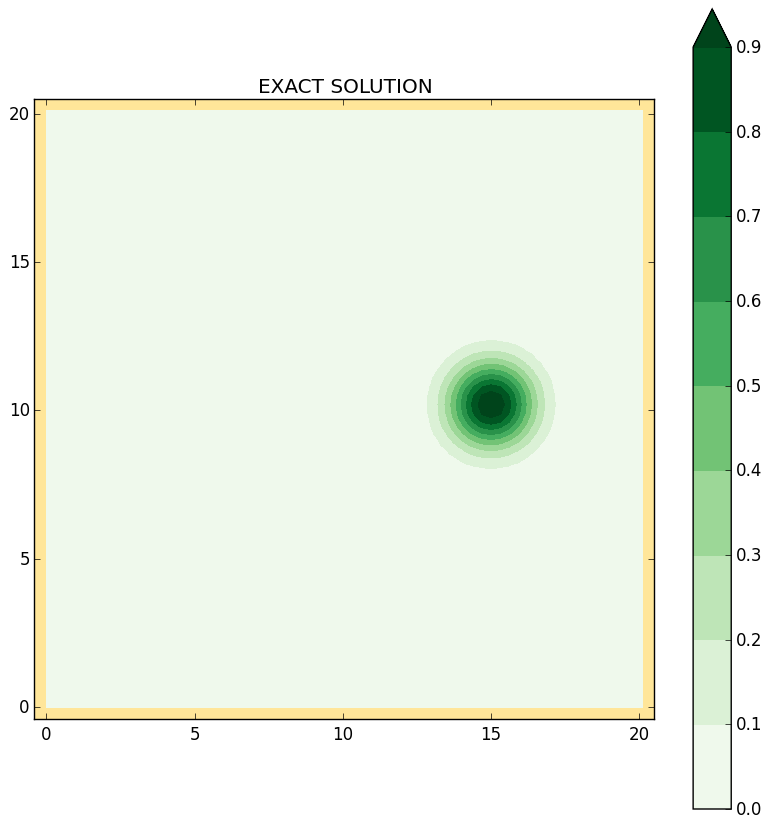
\includegraphics[trim=19mm 19mm 35mm 21mm,clip,scale=0.28]{../img/figure_EX.png}
\end{minipage}%
\begin{minipage}[t]{0.50\textwidth}
 \centering
 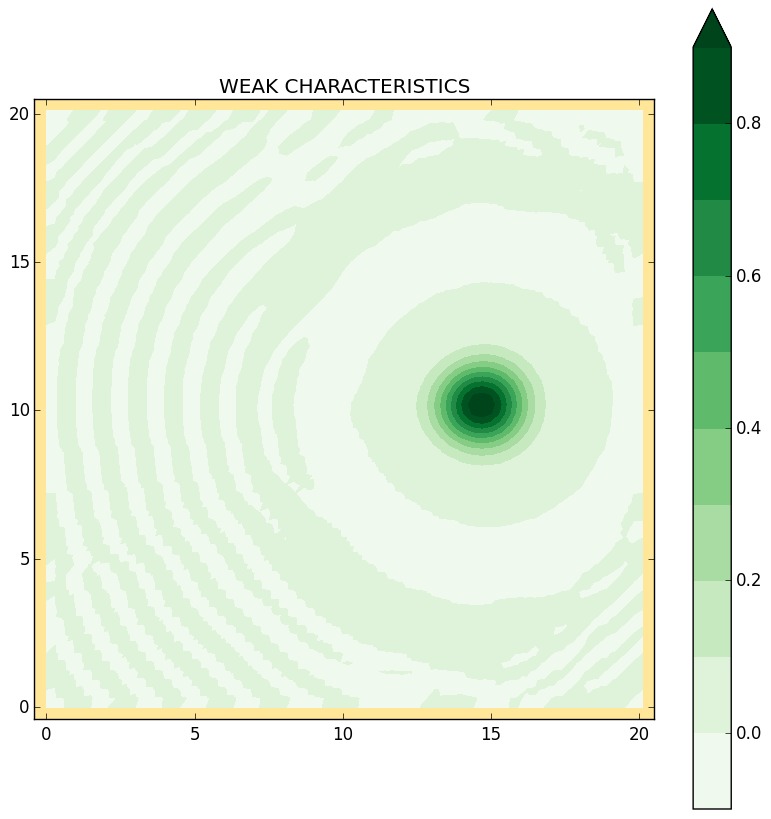
\includegraphics[trim=19mm 19mm 35mm 21mm,clip,scale=0.28]{../img/figure_WC.png}
\end{minipage}
\begin{minipage}[t]{0.50\textwidth}
 \centering
 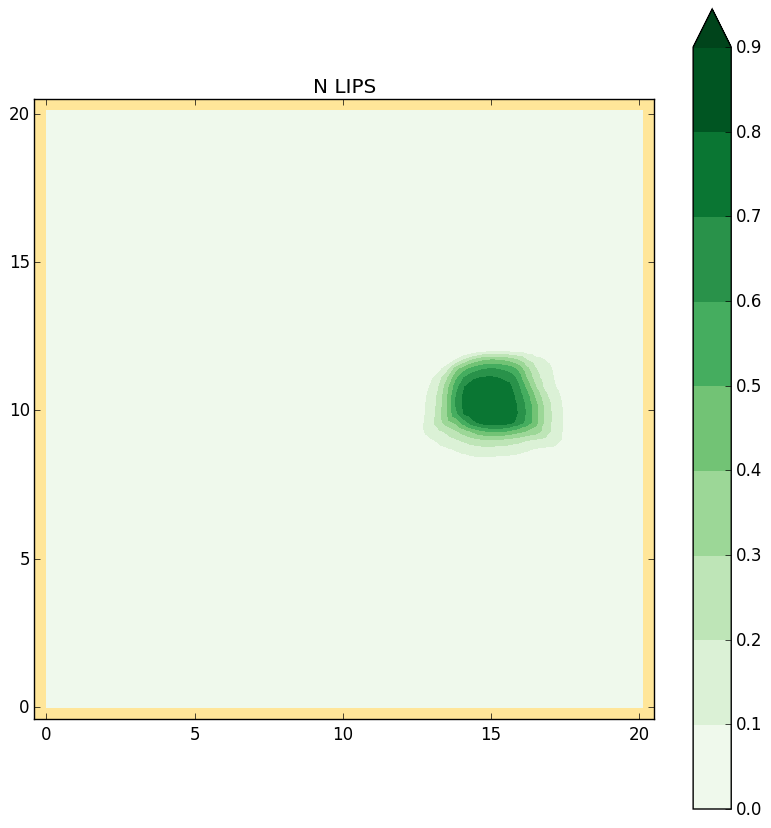
\includegraphics[trim=19mm 19mm 35mm 21mm,clip,scale=0.28]{../img/figure_LIN.png}
\end{minipage}%
\begin{minipage}[t]{0.50\textwidth}
 \centering
 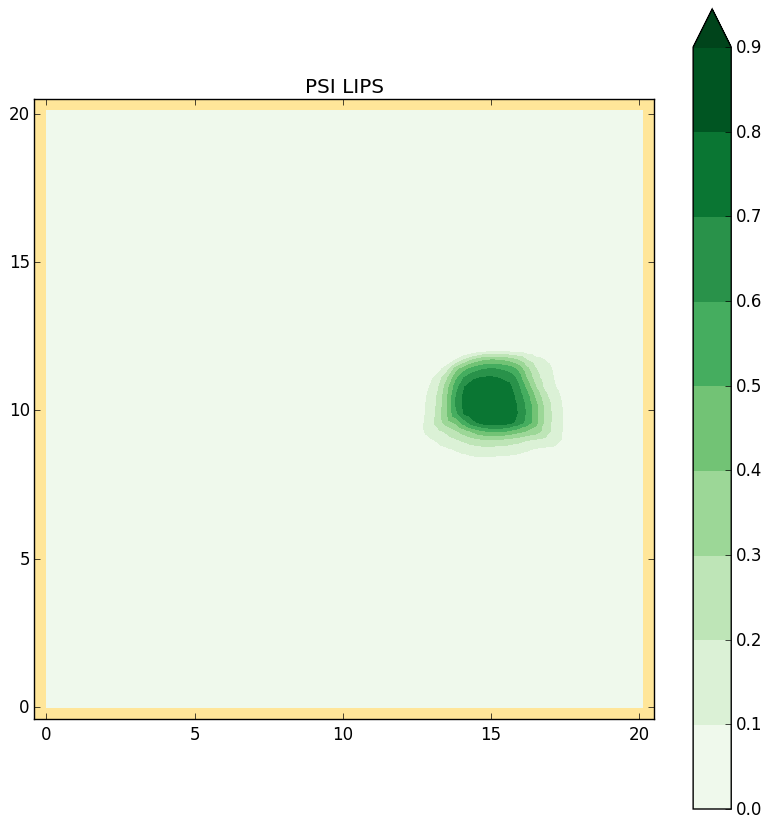
\includegraphics[trim=19mm 19mm 35mm 21mm,clip,scale=0.28]{../img/figure_LIPS.png}
\end{minipage}
\begin{minipage}[t]{0.50\textwidth}
 \centering
 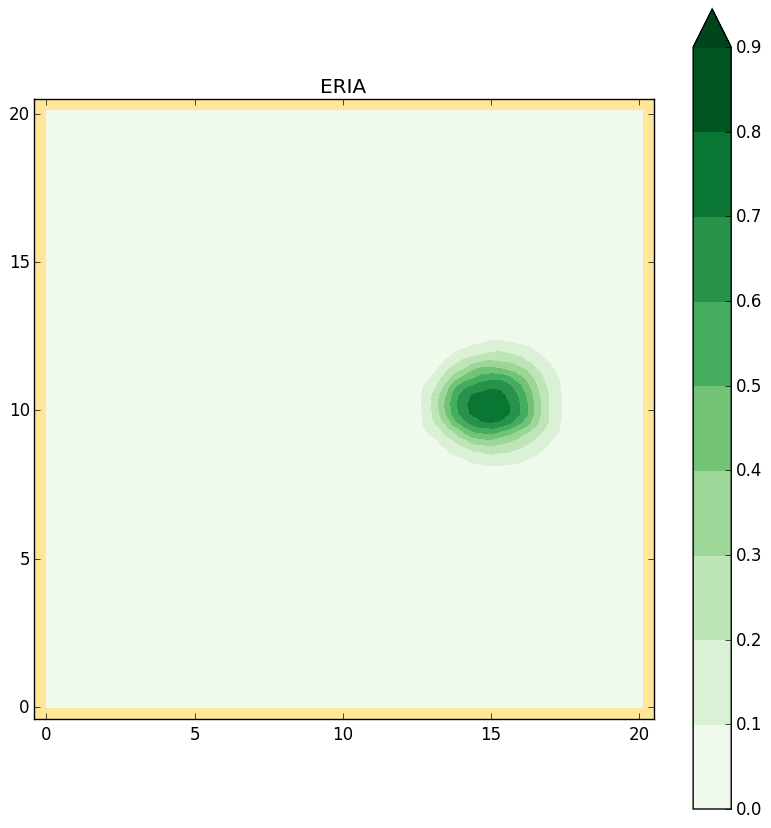
\includegraphics[trim=19mm 19mm 35mm 21mm,clip,scale=0.28]{../img/figure_ERIA.png}
\end{minipage}%
\begin{minipage}[t]{0.50\textwidth}
 \centering
 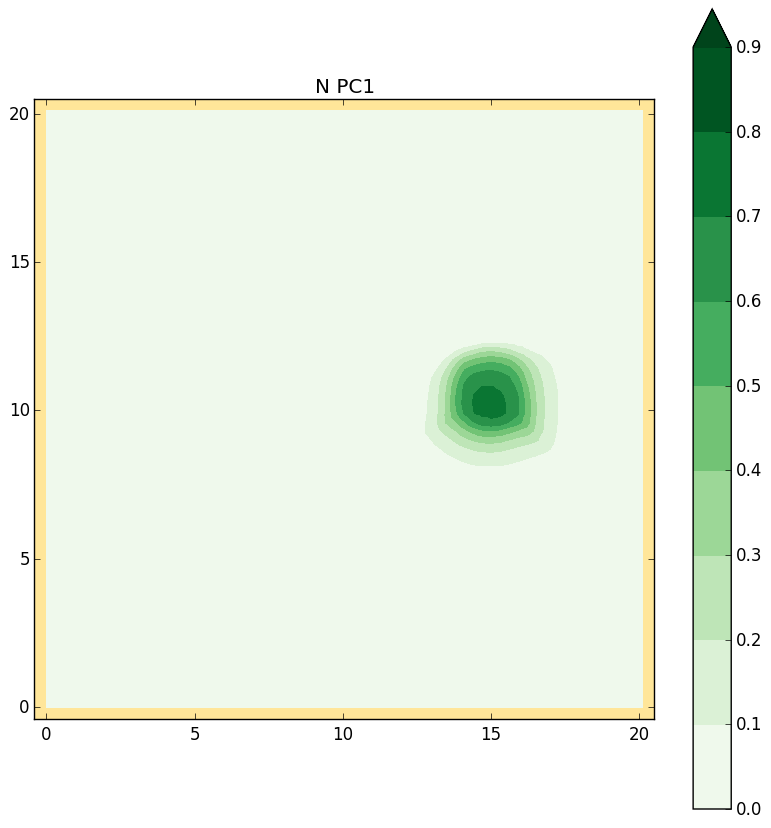
\includegraphics[trim=19mm 19mm 35mm 21mm,clip,scale=0.28]{../img/figure_PC_N1.png}
\end{minipage}
\begin{minipage}[t]{0.50\textwidth}
 \centering
 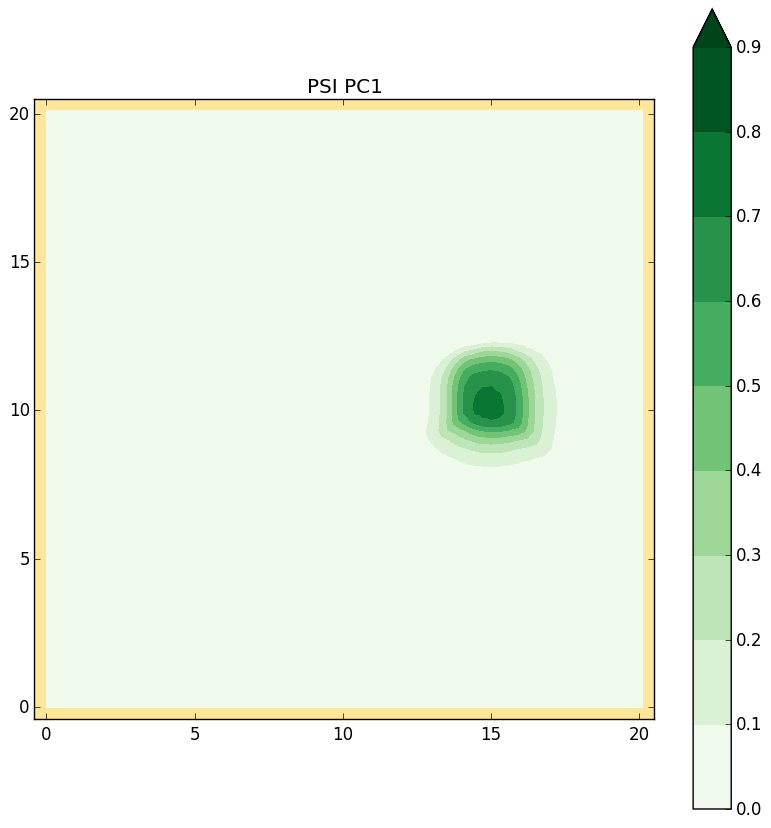
\includegraphics[trim=19mm 19mm 35mm 21mm,clip,scale=0.28]{../img/figure_PC_PSI1.png}
\end{minipage}%
\begin{minipage}[t]{0.50\textwidth}
 \centering
 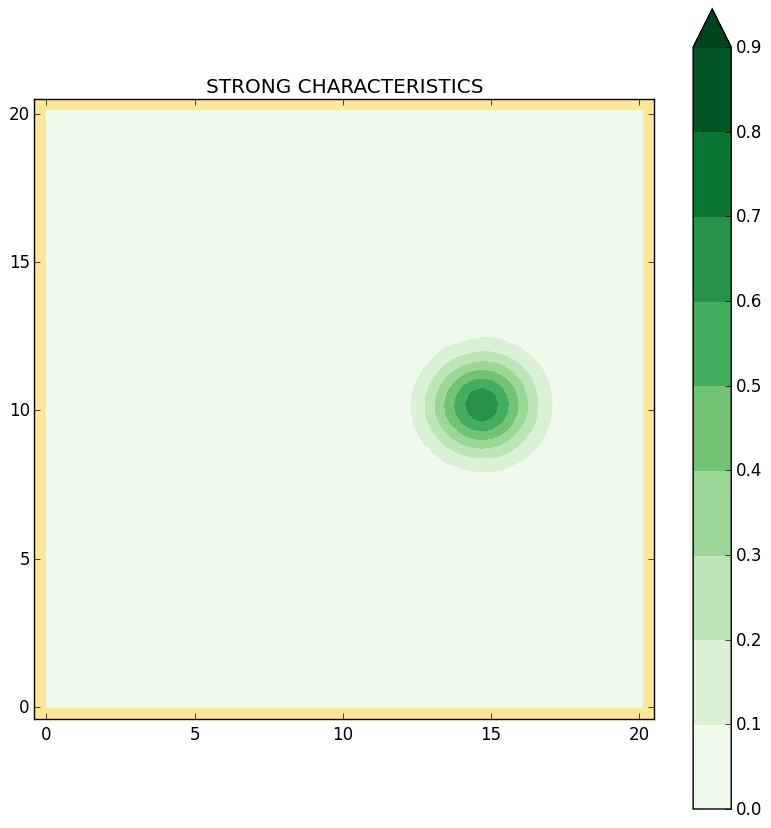
\includegraphics[trim=19mm 19mm 35mm 21mm,clip,scale=0.28]{../img/figure_SC.png}
\end{minipage}
 \caption{Cone test: contour lines of gaussian tracer functions after one period of rotation, for the advection schemes of \telemac{2d}.}
 \label{t2d:cone:profiles1}
\end{figure}
\begin{figure}[h!]
\begin{minipage}[t]{0.50\textwidth}
 \centering
 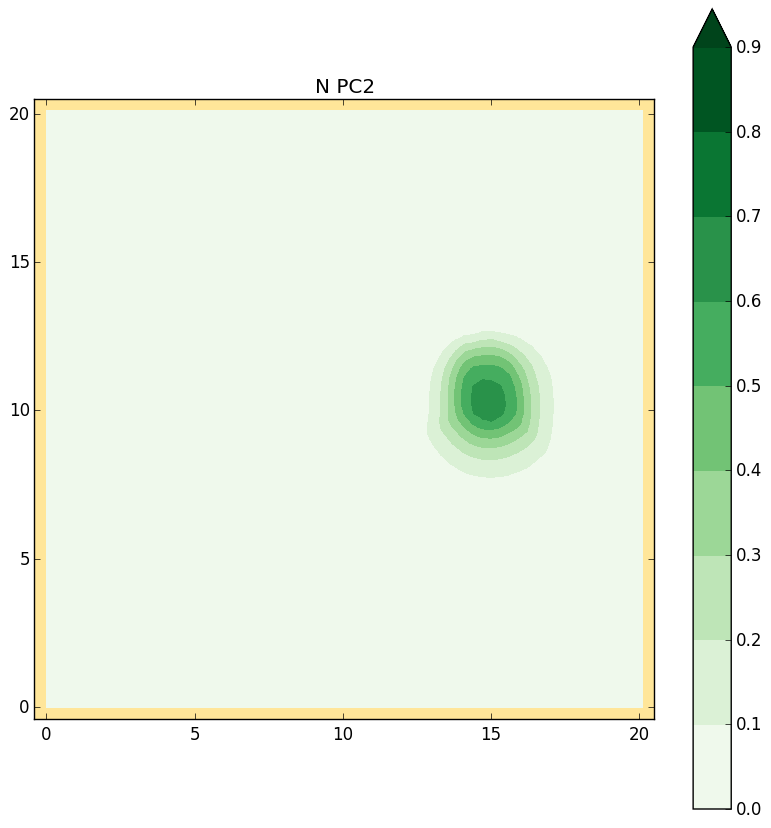
\includegraphics[trim=19mm 19mm 35mm 21mm,clip,scale=0.28]{../img/figure_PC_N2.png}
\end{minipage}%
\begin{minipage}[t]{0.50\textwidth}
 \centering
 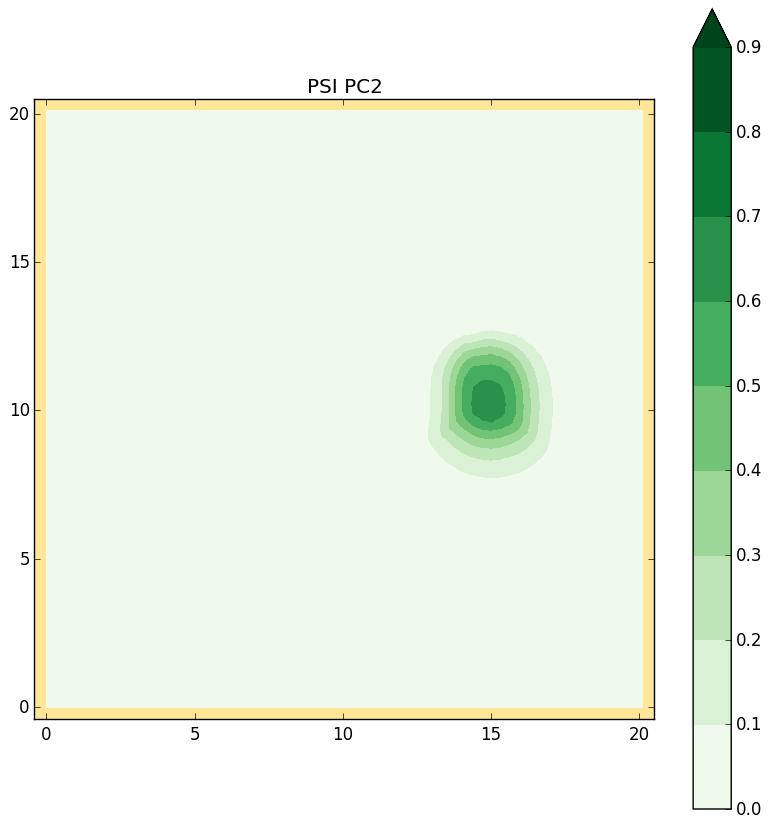
\includegraphics[trim=19mm 19mm 35mm 21mm,clip,scale=0.28]{../img/figure_PC_PSI2.png}
\end{minipage}
\begin{minipage}[t]{0.50\textwidth}
 \centering
 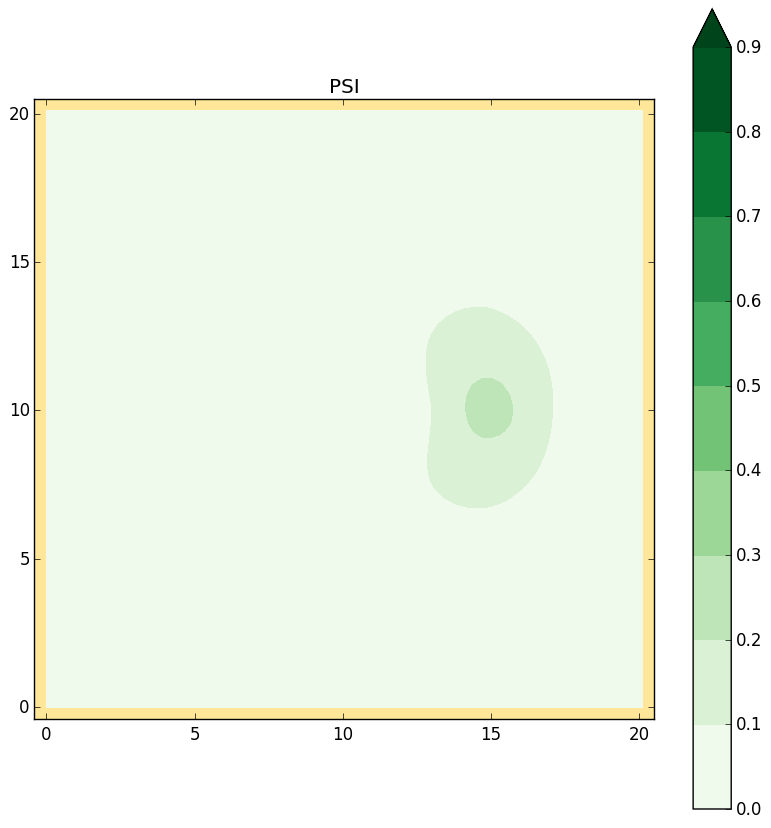
\includegraphics[trim=19mm 19mm 35mm 21mm,clip,scale=0.28]{../img/figure_PSI.png}
\end{minipage}%
\begin{minipage}[t]{0.50\textwidth}
 \centering
 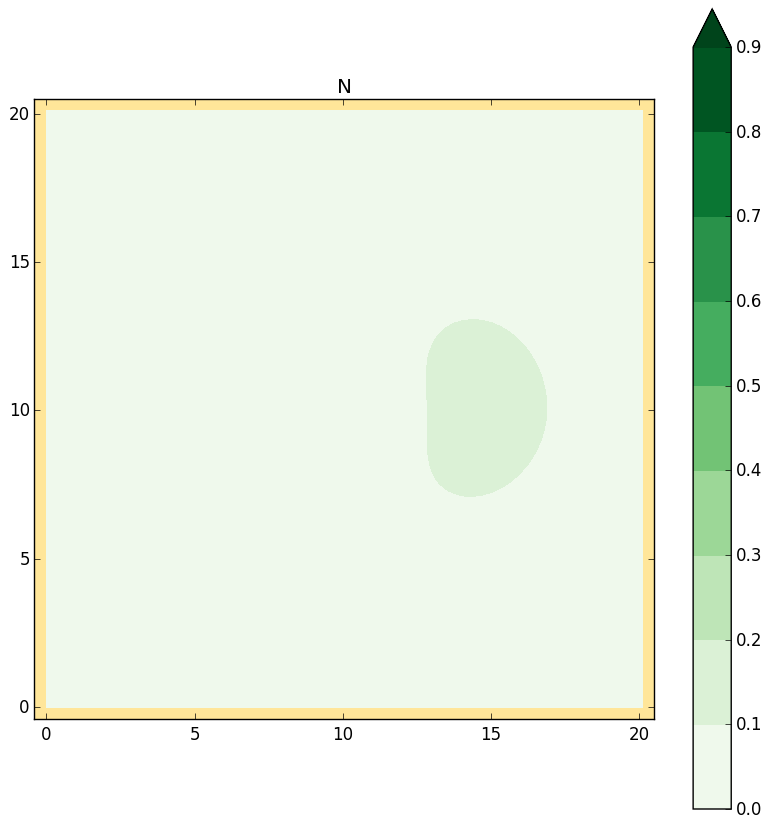
\includegraphics[trim=19mm 19mm 35mm 21mm,clip,scale=0.28]{../img/figure_N.png}
\end{minipage}
 \caption{Cone test: contour lines of gaussian tracer functions after one period of rotation, for the advection schemes of \telemac{2d}.}
 \label{t2d:cone:profiles2}
\end{figure}
